\begin{topic}{young-diagram}{Young diagram}
    Given a \tref{integer-partition}{partition} $\lambda = (\lambda_1, \lambda_2, \ldots, \lambda_k)$ of a non-negative integer $n$, a \textbf{Young diagram} of shape $\lambda$ is a collection of $n$ boxes, arranged in left-aligned rows, such that row $i$ has $\lambda_i$ boxes. For example, a Young diagram of shape $(5, 3, 2)$ is given by:
    \[ 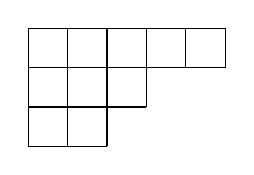
\begin{tikzpicture}
        \begin{scope}[scale=0.5]
            \draw (0, 3) -- (5, 3); \draw (0, 2) -- (5, 2); \draw (0, 1) -- (3, 1); \draw (0, 0) -- (2, 0); \draw (0, 3) -- (0, 0); \draw (1, 3) -- (1, 0); \draw (2, 3) -- (2, 0); \draw (3, 3) -- (3, 1); \draw (4, 3) -- (4, 2); \draw (5, 3) -- (5, 2);
        \end{scope}
    \end{tikzpicture} \]
    The \textit{arm length} of a box $s$, denoted $a_\lambda(s)$, is the number of boxes to the right of $s$. The \textit{leg length} of $s$, denoted $l_\lambda(s)$, is the number of boxes below $s$. The \textit{hook length} $s$ is $a_\lambda(s) + l_\lambda(s) + 1$.
    
    A \textbf{Young tableau} on a Young diagram is a numbering of the boxes by the integers $1, 2, \ldots, n$.
    % A Young tableau is \textbf{standard} if the entries in each row and each column are increasing.
\end{topic}

\begin{topic}{generating-function}{generating function}
    The \textbf{generating function} of a sequence $a_0, a_1, a_2, \ldots$ in a \tref{AA:ring}{commutative ring} $R$ is the formal power series
    \[ \sum_{n = 0}^{\infty} a_n t^n = a_0 + a_1 t + a_2 t^2 + \cdots \in R \llbracket t \rrbracket . \]
\end{topic}

\begin{example}{generating-function}
    \begin{itemize}
        \item The generating function of the constant sequence $1, 1, 1, \ldots$ is
        \[ \sum_{n = 0}^{\infty} t^n = \frac{1}{1 - t} . \]
        \item The generating function of the linear sequence $0, 1, 2, 3, \ldots$ is
        \[ \sum_{n = 0}^{\infty} n t^{n} = t \cdot \frac{d}{dt} \sum_{n = 0}^{\infty} t^{n} = t \cdot \frac{d}{dt} \left( \frac{1}{1 - t} \right) = \frac{t}{(1 - t)^2} . \]
        \item Consider the Fibonacci numbers given by $F_0 = 0, F_1 = 1$ and $F_n = F_{n - 1} + F_{n - 2}$ for $n \ge 2$, and let $f = \sum_{n \ge 0} F_n t^n \in \ZZ \llbracket t \rrbracket$. The recurrence relation implies that
        \[ (1 - t - t^2) f = F_0 + (F_1 - F_0) t + \sum_{n \ge 2} (F_n - F_{n - 1} - F_{n - 2}) t^n = t , \]
        so that $f = t / (1 - t - t^2)$.
    \end{itemize}
\end{example}

\begin{example}{generating-function}
    Assuming $R$ has \tref{AA:characteristic}{characteristic} zero, the sequence can be obtained from the generating function $F \in R \llbracket t \rrbracket$ as follows. Writing
    \[ F = \sum_{n = 0}^{\infty} a_n t^n = a_0 + a_1 t + a_2 t^2 + \cdots , \]
    we obtain the coefficients $a_n$ from the $n$-th derivatives of $F$ as
    \[ a_n = \frac{F^{(n)}(0)}{n!} . \]
\end{example}

\begin{topic}{mobius-function}{Möbius function}
    The \textbf{Möbius function} $\mu$ is the function that assigns to any positive integer $n > 0$ the value
    \[ \mu(n) = \sum_{\substack{1 \le k \le n \\ \gcd(k, n) = 1}} e^{2\pi i \frac{k}{n}} , \]
    or alternatively,
    \[ \mu(n) = \left\{ \begin{array}{cl}
         +1 & \textup{ if $n$ is square-free with even number of prime factors}, \\
         -1 & \textup{ if $n$ is square-free with odd number of prime factors}, \\
         0 & \textup{ if $n$ has a squared prime factor}.
    \end{array} \right. \]
\end{topic}

\begin{example}{mobius-function}
    The first few values of $\mu$ are given by
    \[ \begin{array}{lllll}
        \mu(1) = 1, & \mu(2) = -1, & \mu(3) = -1, & \mu(4) = 0, & \mu(5) = -1, \\
        \mu(6) = 1, & \mu(7) = -1, & \mu(8) = 0, & \mu(9) = 0, & \mu(10) = 1, \ldots
    \end{array} \]
\end{example}

\begin{topic}{schur-function}{Schur function}
    Let $n$ be a positive integer. Write $a_\alpha = \det(x_i^{\alpha_j})_{i, j = 1}^{n}$ for any sequence $\alpha = (\alpha_1, \ldots, \alpha_n)$. For any partition $\lambda = (\lambda_1, \ldots, \lambda_n)$ of length at most $n$, the \textbf{Schur polynomial} of $\lambda$ is the \tref{AA:symmetric-polynomial}{polynomial}
    \[ s_\lambda = a_{\lambda + \delta} / a_\delta \in \ZZ[x_1, \ldots, x_n] , \]
    where $\delta = (n - 1, n - 2, \ldots, 1, 0)$.
    
    In passing from $n$ to $n + 1$, it can be seen that $s_\lambda(x_1, x_2, \ldots, x_n, 0) = s_\lambda(x_1, x_2, \ldots, x_n)$. Hence, there is a uniquely defined element
    \[ s_\lambda \in \Lambda := \bigoplus_{r \ge 0} \Lambda^r , \quad \textup{ where  } \Lambda^r = \varprojlim_n \ZZ[x_1, \ldots, x_n]_{(r)}^{S_n} , \]
    called the \textbf{Schur function} of $\lambda$.
\end{topic}

\begin{example}{schur-function}
    For $n = 3$, we have
    \begin{itemize}
        \item $s_{(0, 0, 0)} = 1$,
        \item $s_{(1, 0, 0)} = x_1 + x_2 + x_3$,
        \item $s_{(1, 1, 0)} = x_1 x_2 + x_1 x_3 + x_2 x_3$,
        \item $s_{(1, 1, 1)} = x_1 x_2 x_3$,
        \item $s_{(2, 0, 0)} = x_1^2 + x_1 x_2 + x_1 x_3 + x_2^2 + x_2 x_3 + x_3^2$,
        \item $s_{(2, 1, 0)} = (x_1 + x_2) (x_1 + x_3) (x_2 + x_3)$.
    \end{itemize}
    For any $n \ge 1$ and $\lambda = (1, 0, 0, \ldots)$, we have $s_\lambda = \sum_{i = 1}^{n} x_i$, so we obtain the Schur function $s_\lambda = \sum_{i = 1}^{\infty} x_i \in \Lambda$.
\end{example}

% \begin{topic}{macdonald-polynomials}{Macdonald polynomials}
%     Let $q$ and $t$ be two parameters.
    
%     The \textbf{Macdonald polynomials} are a family of polynomials $P_\lambda(q, t)$ uniquely determined by the conditions
%     \[ P_\lambda(q, t) = m_\lambda + \sum_{\mu < \lambda} m_\mu \]
%     \[ \langle P_\lambda, P_\mu \rangle_{q, t} = 0 \quad \textup{ for } \lambda \ne \mu . \]
%     where
%     \[ \langle p_\lambda, p_\mu \rangle = \delta_{\lambda \mu} z_\lambda \prod_{i = 1}^{\ell(\lambda)} \frac{1 - q^{\lambda_i}}{1 - t^{\lambda_i}} . \]
% \end{topic}

\begin{topic}{hall-inner-product}{Hall inner product}
    Let $\Lambda$ be the ring of symmetric polynomials in infinitely many variables. For any \tref{GM:integer-partition}{partition} $\lambda = (\lambda_1, \ldots, \lambda_n)$, let $m_\lambda \in \Lambda$ and $h_\lambda \in \Lambda$ denote the \tref{AA:symmetric-polynomial}{monomial and homogeneous symmetric polynomials} in infinitely many variables, respectively. It can be shown that both $\{ m_\lambda \}$ and $\{ h_\lambda \}$ form a $\ZZ$-basis of $\Lambda$.
    
    The \textbf{Hall inner product} is the symmetric bilinear map given by
    \[ \langle \cdot, \cdot \rangle : \Lambda \times \Lambda \to \Lambda, \qquad \langle m_\lambda, h_\mu \rangle = \delta_{\lambda \mu} . \]
\end{topic}

\begin{example}{hall-inner-product}
    The \tref{schur-function}{Schur functions} $\{ s_\lambda \}$ also form a $\ZZ$-basis for $\Lambda$, and moreover, an orthogonal $\ZZ$-basis:
    \[ \langle s_\lambda, s_\mu \rangle = \delta_{\lambda \mu} \quad \textup{ for all } \lambda, \mu . \]
\end{example}

\begin{topic}{binomial-theorem}{binomial theorem}
    Let $R$ be a \tref{AA:ring}{commutative ring}. The \textbf{binomial theorem} states that
    \[ (x + y)^n = \sum_{k = 0}^{n} \binom{n}{k} x^{n - k} y^k \]
    for all $x, y \in R$ and any integer $n \ge 0$.
\end{topic}

\begin{topic}{integer-partition}{integer partition}
    A \textbf{partition} of a non-negative integer $n$ is a tuple of integers $\lambda = (\lambda_1, \ldots, \lambda_k)$ such that $\lambda_1 + \cdots + \lambda_k = n$ and $\lambda_1 \ge \cdots \ge \lambda_k \ge 0$.
\end{topic}

\begin{example}{integer-partition}
    There are $7$ partitions of $5$:
    \begin{itemize}
        \item $5 = 1 + 1 + 1 + 1 + 1$,
        \item $5 = 2 + 1 + 1 + 1$,
        \item $5 = 2 + 2 + 1$,
        \item $5 = 3 + 1 + 1$,
        \item $5 = 3 + 2$,
        \item $5 = 4 + 1$,
        \item $5 = 5$.
    \end{itemize}
\end{example}

\begin{example}{integer-partition}
    The numbers $p_n$ of partitions of $n$ can be collected in a \tref{generating-function}{generating function}
    \[ P(t) = \sum_{n \ge 0} p_n t^n = \prod_{i = 1}^{\infty} \frac{1}{1 - t^i} \in \ZZ \llbracket t \rrbracket . \]
\end{example}

\begin{topic}{conjugate-partition}{conjugate partition}
    Given a \tref{integer-partition}{partition} $\lambda = (\lambda_1, \ldots, \lambda_k)$ of a non-negative integer $n$, the \textbf{conjugate partition} $\lambda' = (\lambda'_1, \ldots, \lambda'_\ell)$ to $\lambda$ is given by
    \[ \lambda'_i = | \{ 1 \le j \le k \mid \lambda_j \ge i \} | \]
    for $1 \le i \le \ell$, where $\ell = \lambda_1$.
\end{topic}

\begin{example}{conjugate-partition}
    The conjugate partition to $\lambda = (5, 3, 2)$ is $\lambda' = (3, 3, 2, 1, 1)$. Note that the \tref{young-diagram}{Young diagram} corresponding to a conjugate partition $\lambda'$ is the transpose of the Young diagram corresponding to $\lambda$.
    \[ 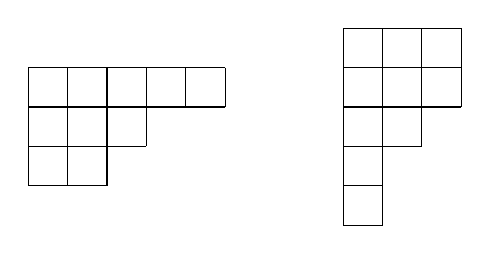
\begin{tikzpicture}
        \begin{scope}[scale=0.5]
            \draw (0, 3) -- (5, 3); \draw (0, 2) -- (5, 2); \draw (0, 1) -- (3, 1); \draw (0, 0) -- (2, 0); \draw (0, 3) -- (0, 0); \draw (1, 3) -- (1, 0); \draw (2, 3) -- (2, 0); \draw (3, 3) -- (3, 1); \draw (4, 3) -- (4, 2); \draw (5, 3) -- (5, 2);
        \end{scope}
        \begin{scope}[scale=0.5, shift={(8, -1)}]
            \draw (0, 5) -- (3, 5); \draw (0, 4) -- (3, 4); \draw (0, 3) -- (3, 3); \draw (0, 2) -- (2, 2); \draw (0, 1) -- (1, 1); \draw (0, 0) -- (1, 0); \draw (0, 0) -- (0, 5); \draw (1, 0) -- (1, 5); \draw (2, 2) -- (2, 5); \draw (3, 3) -- (3, 5);
        \end{scope}
    \end{tikzpicture}\]
\end{example}

\begin{topic}{zorns-lemma}{Zorn's lemma}
    Let $P$ be a \tref{ST:partial-order}{partially ordered set}, such that every chain in $P$
    \[ x_1 \le x_2 \le x_3 \le \cdots \]
    has an upper bound in $P$. Then \textbf{Zorn's lemma} states that $P$ contains at least one maximal element.
\end{topic}

\begin{topic}{fermat-little-theorem}{Fermat's little theorem}
    Let $p$ be a prime number and $a$ an integer. \textbf{Fermat's little theorem} states that
    \[ a^p \equiv a \mod p . \]
\end{topic}

\begin{example}{fermat-little-theorem}
    \begin{proof}
        For $a \equiv 0 \mod p$ the proof is trivial. Otherwise, the order of $a \mod p \in (\ZZ/p\ZZ)^*$ divides the order of the group, which is $p - 1$, so it follows that $a^{p - 1} \equiv 1 \mod p$, and hence $a^p \equiv a \mod p$.
    \end{proof}
\end{example}

\begin{topic}{equivalence-relation}{equivalence relation}
    Let $X$ be a set. An \textbf{equivalence relation} on $X$ is a \tref{ST:binary-relation}{binary relation} $\sim$ on $X$ such that
    \begin{itemize}
        \item (\textit{reflexivity}) $x \sim x$ for all $x \in X$,
        \item (\textit{symmetry}) $x \sim y$ if and only if $y \sim x$ for all $x, y \in X$,
        \item (\textit{transitivity}) if $x \sim y$ and $y \sim z$, then $x \sim z$ for all $x, y, z \in X$.
    \end{itemize}
\end{topic}

\begin{topic}{pascal-rule}{Pascal's rule}
    \textbf{Pascal's rule} states that
    \[ \binom{n}{k} = \binom{n - 1}{k} + \binom{n - 1}{k - 1} \]
    for all integers $n, k \ge 1$.
\end{topic}

\begin{topic}{lagrange-polynomial}{Lagrange polynomial}
    Given $k + 1$ distinct numbers $x_0, \ldots, x_k$, the \textbf{Lagrange basis polynomials} are the polynomials
    \[ \ell_j(x) = \prod_{\substack{0 \le i \le k \\ i \ne j}} \frac{x - x_i}{x_j - x_i} . \]
    Given $k + 1$ values $y_0, \ldots, y_k$, the \textbf{Lagrange interpolating polynomial} through the points $(x_0, y_0), \ldots, (x_k, y_k)$ is the polynomial
    \[ L(x) = \sum_{j = 0}^{k} y_j \ell_j(x) . \]
\end{topic}

\begin{example}{lagrange-polynomial}
    Consider the three points $(2, 1), (3, 5)$ and $(5, 19)$. The Lagrange basis polynomials are
    \[ \begin{aligned}
        \ell_0(x) &= \frac{(x - 3)(x - 5)}{(2 - 3)(2 - 5)} = \tfrac{1}{3} (x - 5)(x - 3) , \\
        \ell_1(x) &= \frac{(x - 2)(x - 5)}{(3 - 2)(3 - 5)} = -\tfrac{1}{2} (x - 5)(x - 2) , \\
        \ell_2(x) &= \frac{(x - 2)(x - 3)}{(5 - 2)(5 - 3)} = \tfrac{1}{6} (x - 3)(x - 2) .
    \end{aligned} \]
    Hence, the Lagrange interpolation polynomial is
    \[ L(x) = \ell_0(x) + 5 \ell_1(x) + 19 \ell_2(x) = x^2 - x - 1 . \]
\end{example}

\begin{topic}{continued-fraction}{continued fraction}
    Let $x \in \RR$ be a real number. The \textbf{continued fraction} of $x$ is a (possibly finite) sequence
    \[ [a_0; a_1, a_2, \ldots] \]
    given by $a_i = \lfloor x_i \rfloor$ with $x_0 = x$ and $x_{i + 1} = \frac{1}{x_i - a_i}$. The sequence stops if $x_i = a_i$, which happens precisely if $x$ is rational.
    
    The continued fraction of $x$ is also commonly denoted as
    \[ x = a_0 + \frac{1}{a_1 + \frac{1}{a_2 + \frac{1}{a_3 + \cdots }}} . \]
\end{topic}

\begin{example}{continued-fraction}
    \begin{itemize}
        \item $\sqrt{2} = [1; 2, 2, 2, 2, 2, 2, \ldots]$
        \item $2/7 = [0; 3, 2]$
        \item $e = [2; 1, 2, 1, 1, 4, 1, 1, 6, 1, 1, 8, \ldots]$
        \item $\pi = [3; 7, 15, 1, 292, 1, 1, 1, 2, 1, 3, 1, \ldots]$
    \end{itemize}
\end{example}

\begin{topic}{dickson-lemma}{Dickson's lemma}
    For any $n \ge 1$, consider the \tref{ST:partial-order}{partial order} on $\NN^n$ given by
    \[ (a_1, \ldots, a_n) \le (b_1, \ldots, b_n) \iff a_i \le b_i \textup{ for all } i . \]
    \textbf{Dickson's lemma} states that every non-empty subset $S \subset \NN^n$ has only finitely many minimal elements.
\end{topic}

\begin{topic}{mean-value-theorem}{mean value theorem}
    Let $f : [a, b] \to \RR$ be a continuous function, which is differentiable on $(a, b)$. The \textbf{mean value theorem} states that there exists a $c \in (a, b)$ such that
    \[ f'(c) = \frac{f(b) - f(a)}{b - a} . \]
\end{topic}

\begin{topic}{intermediate-value-theorem}{intermediate value theorem}
    Let $f : [a, b] \to \RR$ be a continuous function. The \textbf{intermediate value theorem} states that for every value $y$ between $f(a)$ and $f(b)$, there exists an $x \in [a, b]$ such that $y = f(x)$.
\end{topic}
